\documentclass{article}
\usepackage{svg}
\usepackage{caption}
\usepackage{subcaption}
\usepackage{graphicx}
\usepackage{tabularx}

\usepackage[margin=1in]{geometry} % for 1 inch side panels


\begin{document}

\begin{titlepage}
    \centering
    \vspace*{0cm}
    {\scshape\Large Frankfurt University of Applied Sciences}\\[3cm]
    {\huge\bfseries Title}\\[8cm]
    {\Large\itshape Group 6:}\\
    {\Large\itshape Hermon Giikael, Howard-Yi Hong Soon, Jiwon Won, Lars Friese, Marc Roemer, Stefan Nguyen}\\[4cm]
    Supervisor:\\
    Jörg Schäfer\\[3cm]
    {\large \today}
\end{titlepage}

\tableofcontents
\newpage

\section{Hermon Gimikael}

	\subsection{Requirement1}
		\begin{figure}[h!]
		    \centering
		    \captionsetup{labelformat=empty}
		    \caption{Your caption}
		    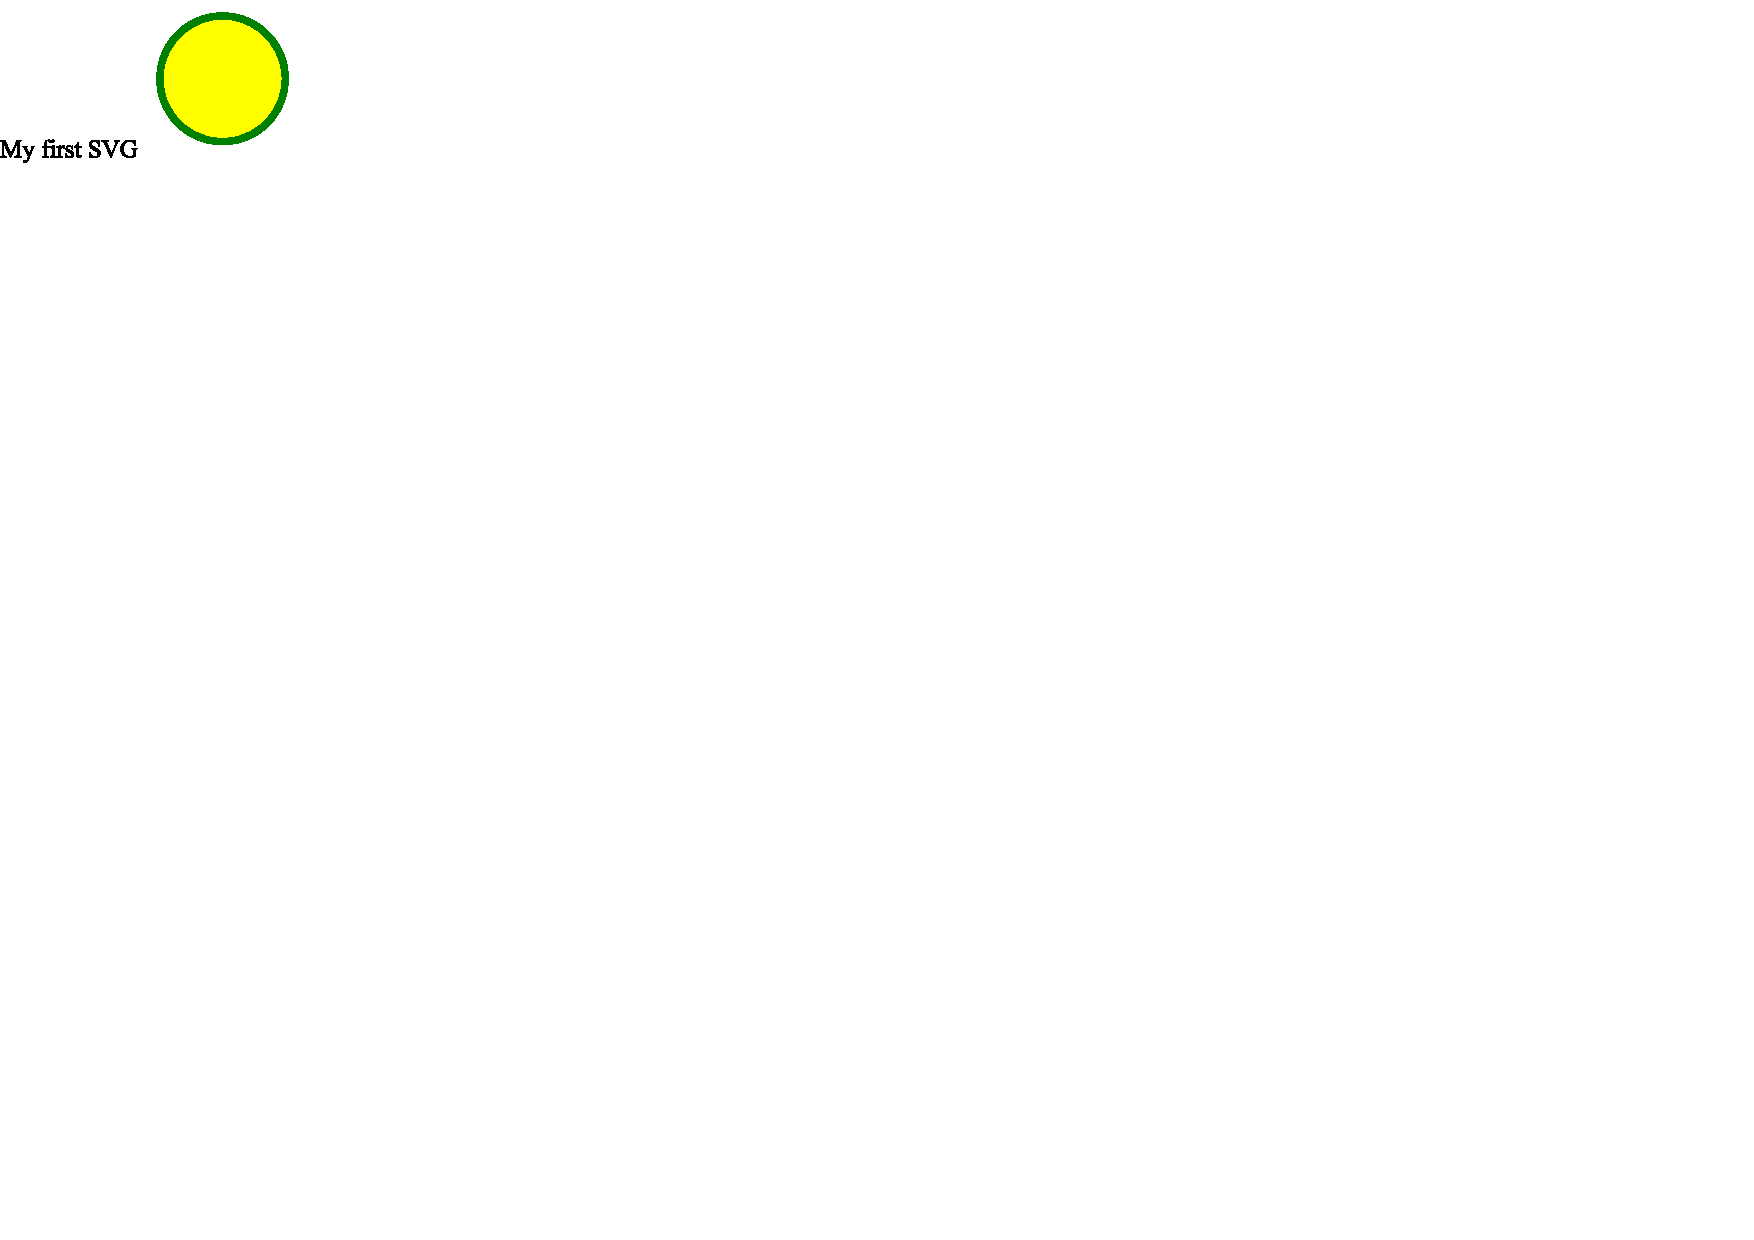
\includegraphics[width=\textwidth, angle=0]{Kreis2.pdf}
		\end{figure}
		\newpage
		\begin{figure}[h!]
		    \centering
		    \captionsetup{labelformat=empty}
		    \caption{Your caption}
		    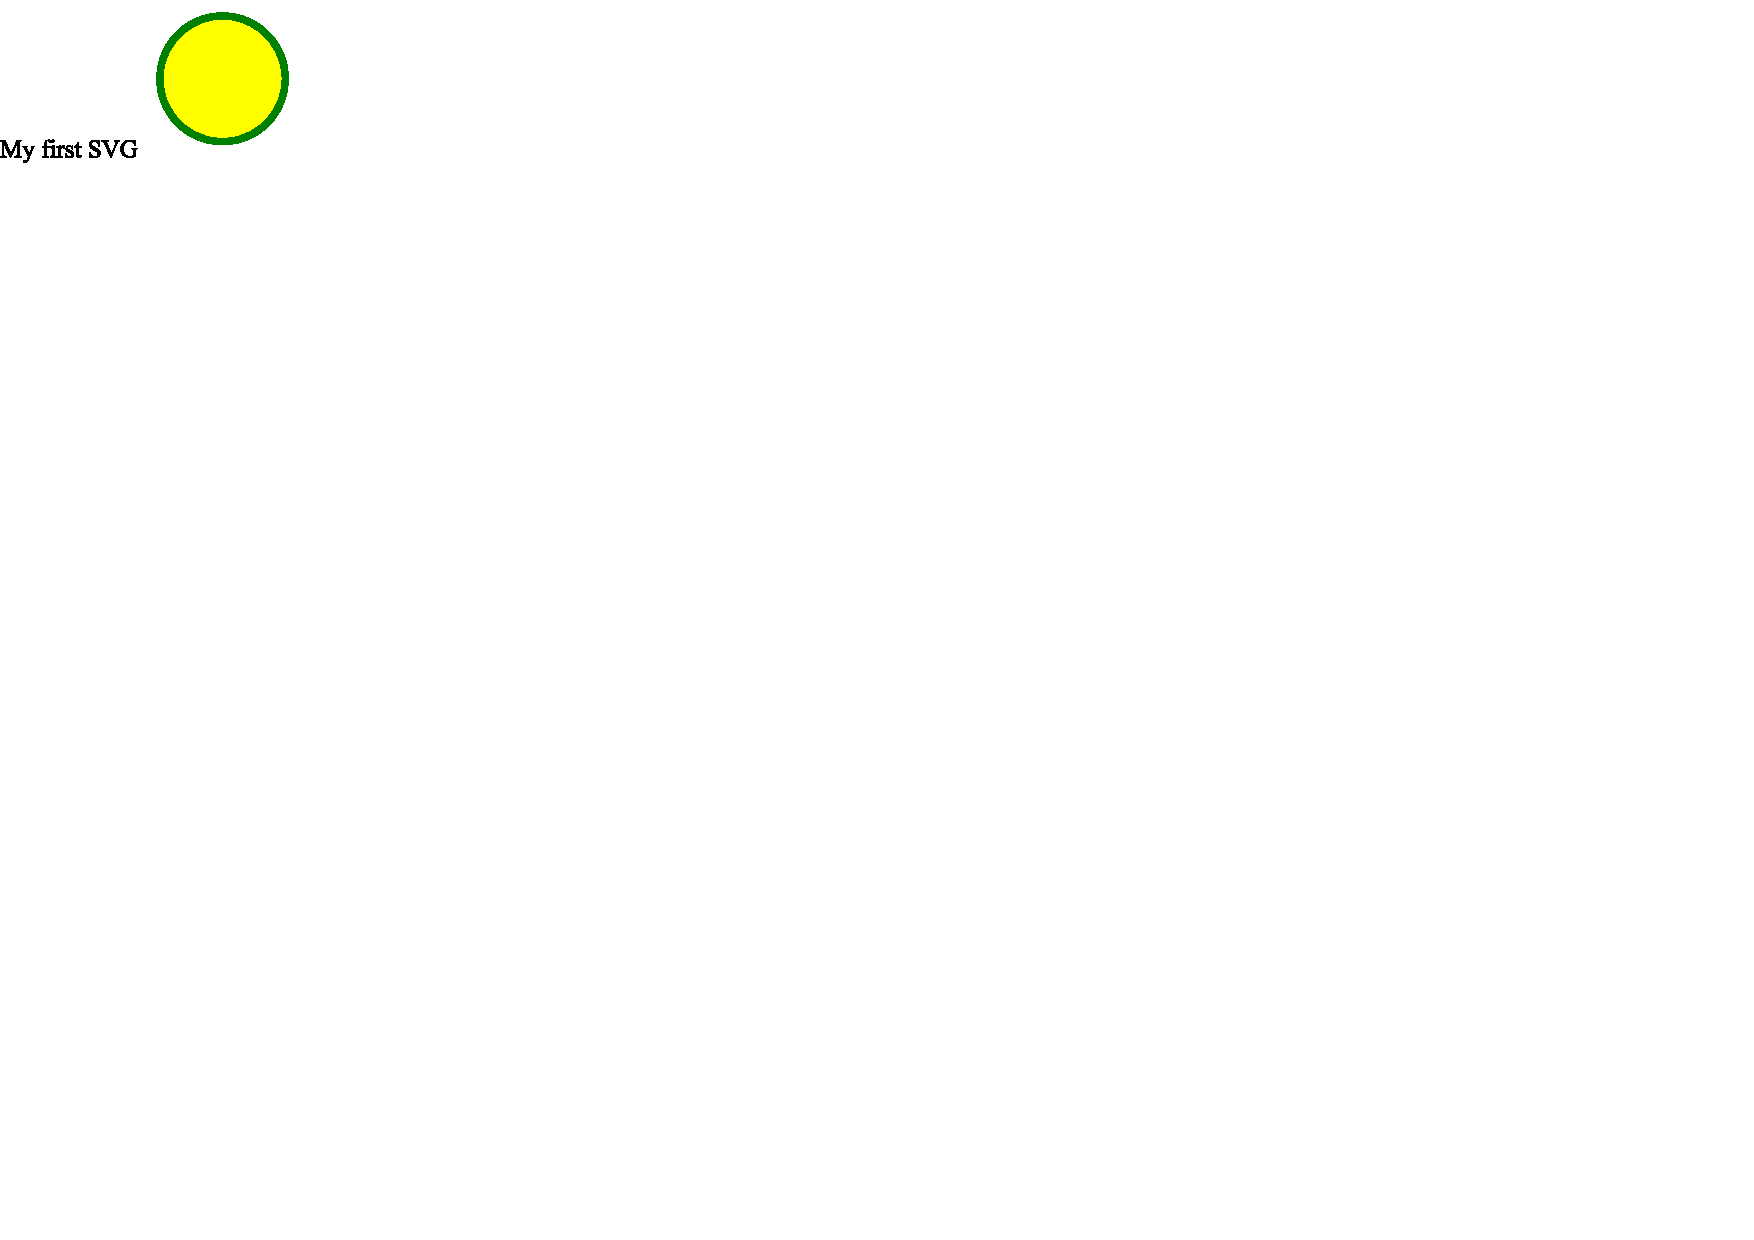
\includegraphics[width=\textwidth, angle=0]{Kreis2.pdf}
		\end{figure}
		\newpage
	
	\subsection{Requirement2}
		\begin{figure}[h!]
		    \centering
		    \captionsetup{labelformat=empty}
		    \caption{Your caption}
		    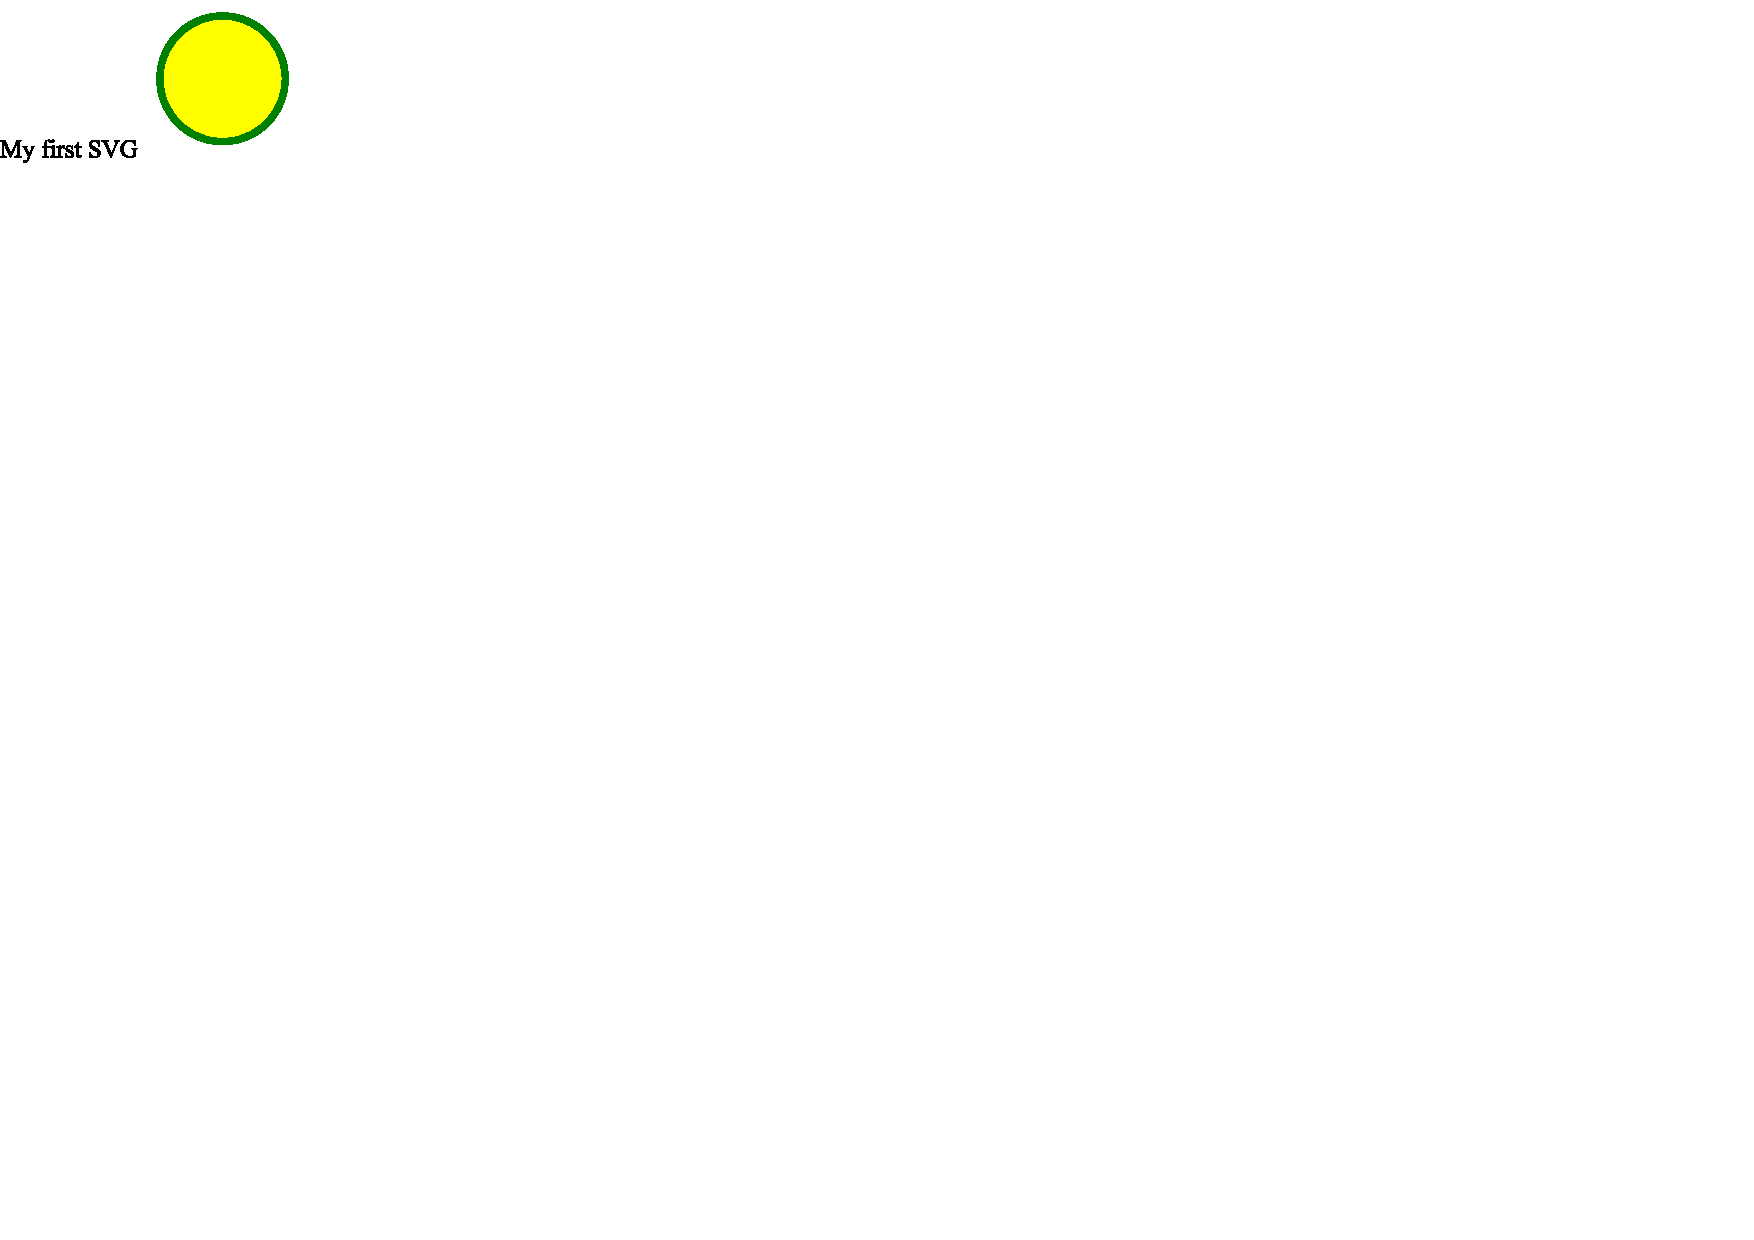
\includegraphics[width=\textwidth, angle=0]{Kreis2.pdf}
		\end{figure}
		\newpage

\section{Howard-Yi Hong Soon}
		\subsection{Requirement 5: Share workout achievement on social media}
		
		\begin{center}
			\begin{tabularx}{1.0\textwidth}{|>{\raggedright\arraybackslash}p{0.2\textwidth}|>{\raggedright\arraybackslash}X|}
				\hline
				Name             & Share workout achievements on social media \\ \hline
				ID               & 5 \\ \hline
				Business Value   & Low \\ \hline
				Description      & Create workout achievements page and share it to logged-in social media \\ \hline
				Trigger          & Push "share" button and chose specific social media to be delivered achievement page\\ \hline
				Actors           & User, Workout System, Social Media System\\ \hline
				Pre-conditions   & User successfully logged in social media, internet connected\\ \hline
				Post-conditions  & User post workout achievement page on social media\\ \hline
				Basic Flow       & \\ \hline
								Description Actions& This is the main scenario when user has an achievement to share and linked social media account \\ \hline
								1 & The use chooses an achievement to share \\ \hline
								2 & The workout system creates the achievement post \\ \hline
								3 & The user chooses a social media app to share \\ \hline
								4 & The workout system sends the achievement post to the social media system \\ \hline
				Alternative Flow & A \\ \hline
								Description Actions& There isn't any achievement to share \\ \hline
								1 & The workout system shows "Start workout and share it" \\ \hline
				Alternative Flow & B \\ \hline
								Description Actions& User does not have a social media app \\ \hline
								1 & The user chooses an achievement to share \\ \hline
								2 & The workout system creates the achievement post \\ \hline
								3 & The user chooses "download image" \\ \hline
								4 & The workout system send the achievement post to the gallery storage\\ \hline
			\end{tabularx}
		\end{center}

		\paragraph{Functional requirements}

		\begin{itemize}
			\item \textbf{The workout system syncs with social media accounts.}
			\item \textbf{The workout system creates an achievement post including user's goal, time, workout type.}
		\end{itemize}
		
		\paragraph{Non-functional requirements}
		
		\begin{itemize}
			\item \textbf{The sharing post is easy to read and compactly designed.}
			\item \textbf{The system is well connected to all social media accounts when the internet is available.}
		\end{itemize}
		
	

	\begin{figure}[htbp]
		\textbf{Howard-Yi Hong Soon}
		\centering
		\begin{subfigure}{\textwidth}
			\resizebox{\textwidth}{!}{\includesvg[]{Howard/share_workout/ShareWorkoutAchievement_usecase.svg}}
			\caption{Use Case Diagram}
		\end{subfigure}
		\begin{subfigure}{\textwidth}
			This ShareWorkoutAchievement use case shows the operations and the interaction between system and user
			of the requirement. It has a few of includes and extends, e.g. display message "start workout and share it" and
			select achievement, the user has to click on share button in order to trigger them. "Share achievement on Social Media" has an extend
			optional function to download image. 
		\end{subfigure}
	\end{figure}
	


	\begin{figure}[htbp]
		\textbf{Howard-Yi Hong Soon}
		\centering
		\begin{subfigure}{\textwidth}
			\resizebox{\textwidth}{!}{\includesvg[]{Howard/share_workout/ShareWorkoutAchievement_activity.svg}}
			\caption{Activity Diagram}
		\end{subfigure}
		\begin{subfigure}{\textwidth}
			This ShareWorkoutAchievement activity diagram shows detail flow chart about the requirement. 
			When user select an achievement, either it displays message "start workout and share it" because user has no 
			achievement, or create the achieveme post if the user has achieveme detected. Afterwards, user can choose a 
			social media app to share or just download image and save to gallery.
		\end{subfigure}
	\end{figure}
	

	\begin{figure}[htbp]
		\textbf{Howard-Yi Hong Soon}
		\centering
		\begin{subfigure}{\textwidth}
			\resizebox{\textwidth}{!}{\includesvg[]{Howard/share_workout/ShareWorkoutAchievement_class.svg}}
			\caption{Class Diagram}
		\end{subfigure}
		\begin{subfigure}{\textwidth}
			This ShareWorkoutAchievement class diagram shows the classes, operations and variables that are created
			for this requirement. A UserWorkout class to get their profile information, then a WorkoutAchievement class to save 
			the achievements from user, or display message "start workout...." if user doesn't have the achievement. 
			Then a ShareMedia class to create post and share it in social media. Lastly an additional function to download image
			as an option for user to save and share their achievement post.
		\end{subfigure}
	\end{figure}
	

	
	\begin{figure}[htbp]
		\textbf{Howard-Yi Hong Soon}
		\centering
		\begin{subfigure}{\textwidth}
			\resizebox{\textwidth}{!}{\includesvg[]{Howard/share_workout/ShareWorkoutAchievement_sequence.svg}}
			\caption{Sequence Diagram}
		\end{subfigure}
		\begin{subfigure}{\textwidth}
			This ShareWorkoutAchievement sequence diagram shows the detail work flow between each classes. After user select the achievement
			WorkoutAchievement class start to collect the achievement record. If user has the achievement, it create post to share, but before that authentication is 
			mandatory for user to access their social media account. Otherwise it display the message "start workout..."
		\end{subfigure}
	\end{figure}
	\newpage

		\textbf{Howard-Yi Hong Soon}
		\subsection{Requirement : Nutritional Tracking for food intake and calorie counting}
		\begin{center}
			
			\begin{table}[htbp]
			\begin{tabularx}{1.0\textwidth}{|>{\raggedright\arraybackslash}p{0.2\textwidth}|>{\raggedright\arraybackslash}X|}
				\hline
				Name             & Nutritional tracking for food intake and calorie counting \\ \hline
				ID               & 8 \\ \hline
				Business Value   & Medium \\ \hline
				Description      & A health and nutrition app which allows the user through scanning the barcode
									to track their daily food intake gives the nutritional informations about the food, counts the calories and gives feedback about the 
									users dietary \\ \hline
				Trigger          & User opens the app to track their food for the day and thus triggers the apps food logging feature\\ \hline
				Actors           & User, nutrition app\\ \hline
				Pre-conditions   & User installed and created an account and the app has access database which contains nutritional\\ \hline
				Post-conditions  & The user gets information's about nutritions of food items and a log of all items which has been scanned\\ \hline
				Basic Flow       & \\ \hline
								Description Actions& This is the main scenario when user creates successful a scanning the barcode \\ \hline
								1 & User scanned the barcode of a food item of his choice \\ \hline
								2 & The app gives the calories, vitamins etc. of the logged food item \\ \hline
								3 & The system logs the scanned item for future uses \\ \hline
				Alternative Flow & A \\ \hline
								Description Actions& The app doesn't scan the barcode of the item \\ \hline
								1 & The app shows an error and gives the user a text box to manually write the barcode number of the searched item \\ \hline
								2 & The system searches the item in the food database and gives the nutritional informations and logs the item for future uses \\ \hline
								Alternative Flow & B \\ \hline
								Description Actions& The searched item is not found in the database and shows an error \\ \hline
								1 & The app requests the user to manually input the nutritional information's about the item \\ \hline
								2 & User has to tip in calories, nutrients, serving size and name of the item and saves it \\ \hline
								3 & The app takes the data through a verification process and adds it to the food database \\ \hline
			\end{tabularx}
		\end{table}
		\end{center}
		\paragraph{Functional requirements}
		\begin{itemize}
			\item User should be able to log their food by searching and selecting from a database.
			\item The System should calculate and display the daily calorie intake based on the logged food
					and provide information about the nutrition.
		\end{itemize}
		
		\paragraph{Non-functional requirements}
		\begin{itemize}
			\item The System has to have an easy and user-friendly interface for easy and uncomplicated use. The System
					has to ensure accuracy in recording and storing the data.
			\item The calculations of the calories and the nutritional feedbacks has to be correct which is ensured by a mechanism 
					for prevention of data manipulation.
		\end{itemize}
	

	\begin{figure}[htbp]
		\textbf{Howard-Yi Hong Soon}
		\centering
		\begin{subfigure}{\textwidth}
			\resizebox{\textwidth}{!}{\includesvg[]{Howard/nutriotinal_tracking/NutritionalTracking_usecase.svg}}
			\caption{Use Case Diagram}
		\end{subfigure}
		\begin{subfigure}{\textwidth}
			This NutritionalTracking usecase diagram shows the user has 3 way to input information of item: scan barcode,
			input barcode number or input nutritional infomation. The input nutritional information method will add the item to database.
			Then system will shows calories, vitamins etc. of the logged food item.
		\end{subfigure}
		\resizebox{300pt}{180pt}{\includesvg[]{Stefan/UI Prototypes/Show nutritient and calories.svg}}
	\end{figure}
	

		\begin{figure}[htbp]
			\textbf{Howard-Yi Hong Soon}
			\centering
			\begin{subfigure}{\textwidth}
				\resizebox{\textwidth}{!}{\includesvg[]{Howard/nutriotinal_tracking/NutritionalTracking_activity.svg}}
				\caption{Activity Diagram}
			\end{subfigure}
			\begin{subfigure}{\textwidth}
				This NutritionalTracking activity diagram shows the flow chart of the requirement. Firstly, user log into the app then scan the barcode.
				If barcode is detected it will display the nutriotinal information directly, if no then use has to input nutritional information about the item
				manually, then add it to datbase. But if no barcode is detected, user has the option to manully input barcode number, then it will display the 
				nutritional information in the end.
			\end{subfigure}
		\end{figure}
		

		\begin{figure}[htbp]
			\textbf{Howard-Yi Hong Soon}
			\centering
			\begin{subfigure}{\textwidth}
				\resizebox{\textwidth}{!}{\includesvg[]{Howard/nutriotinal_tracking/NutritionalTracking_class.svg}}
				\caption{Class Diagram}
			\end{subfigure}
			\begin{subfigure}{\textwidth}
				This NutritionalTracking class diagram shows the classes, operations and variables for the requirement.
				The UserData class obtain the user profile information. Then InputBarcode class will detect the barcode,it also has 
				the option when user manually input barcode number or nutritional image. Next, Nutrition class will access all the nutrional
			\end{subfigure}
		\end{figure}
		

		\begin{figure}[htbp]
			\textbf{Howard-Yi Hong Soon}
			\centering
			\begin{subfigure}{\textwidth}
				\resizebox{\textwidth}{!}{\includesvg[]{Howard/nutriotinal_tracking/NutritionalTracking_sequence.svg}}
				\caption{Sequence Diagram}
			\end{subfigure}
			\begin{subfigure}{\textwidth}
			\end{subfigure}
		\end{figure}
		\newpage

		\textbf{Howard-Yi Hong Soon}
		\subsection{Requirement : Appearance Theme}
		\begin{center}
			\begin{table}[htbp]
			\begin{tabularx}{1.0\textwidth}{|>{\raggedright\arraybackslash}p{0.2\textwidth}|>{\raggedright\arraybackslash}X|}
				\hline
				Name             & Appearance Theme \\ \hline
				ID               &  \\ \hline
				Business Value   & Medium \\ \hline
				Description      & User has option to select Light/Dark Theme for their watch\\ \hline
				Trigger          & Light/Dark theme has been selected\\ \hline
				Actors           & User, Theme system\\ \hline
				Pre-conditions   & Light theme is preset at default\\ \hline
				Post-conditions  & System Interface updated, User preference saved\\ \hline
				Basic Flow       & \\ \hline
								Description Actions& This is the main scenario when user select preference theme \\ \hline
								1 & Select between light and dark themes  \\ \hline
								2 & Apply preset font color/background adjustment on system inferface \\ \hline
								3 & Apply preset contrast adjustment on system inferface \\ \hline
								4 & Apply theme on system interface \\ \hline
				Alternative Flow & A \\ \hline
								Description Actions& User want to adjust contrast level \\ \hline
								1 & The user press on "setting" button \\ \hline
								2 & The user adjust contrast manually \\ \hline
								3 & The system apply new contrast level \\ \hline
								Alternative Flow & B \\ \hline
								Description Actions& User want to reset contrast level to default \\ \hline
								1 & The user press on "reset" button \\ \hline
								2 & The system display confirmation to reset  \\ \hline
								3 & The contrast level is reset to deafult value \\ \hline
								4 & The systema apply preset contrast level \\ \hline
			\end{tabularx}
		\end{table}
		\end{center}
		\paragraph{Functional requirements}
		\begin{itemize}
			\item User should be able start, pause and reset the stopwatch.
			\item The stopwatch has a function to save elapsed time after pause.
		\end{itemize}
		
		\paragraph{Non-functional requirements}
		\begin{itemize}
			\item The System need to have an easy and user-friendly interface for time reading.
			\item The interface need to have visible button on interface for start, pause and reset.
		\end{itemize}
	

	\begin{figure}[htbp]
		\textbf{Howard-Yi Hong Soon}
		\centering
		\begin{subfigure}{\textwidth}
			\resizebox{\textwidth}{!}{\includesvg[]{Howard/AppearenceTheme/AppearenceTheme_usecase.svg}}
			\caption{Use Case Diagram}
		\end{subfigure}
		\begin{subfigure}{\textwidth}
			This appearence theme usecase diagram shows the user has 2 options for theme, light and dark theme. It would
			change to light or dark appearance base on user selection. User also has an option to change contrast level, and also a button to reset it.
		\end{subfigure}
	\end{figure}
	

		\begin{figure}[htbp]
			\textbf{Howard-Yi Hong Soon}
			\centering
			\begin{subfigure}{\textwidth}
				\resizebox{\textwidth}{!}{\includesvg[]{Howard/AppearenceTheme/AppearenceTheme_activity.svg}}
				\caption{Activity Diagram}
			\end{subfigure}
			\begin{subfigure}{\textwidth}
				This appearence theme activity diagram show the flow chart of this requirement, user has two option to select, either white or dark theme.
				Each flow apply preset font color and contrast level, then user can adjust contrast level manually if they want to customize it.
			\end{subfigure}
		\end{figure}
		

		\begin{figure}[htbp]
			\textbf{Howard-Yi Hong Soon}
			\centering
			\begin{subfigure}{\textwidth}
				\resizebox{\textwidth}{!}{\includesvg[]{Howard/AppearenceTheme/AppearenceTheme_class.svg}}
				\caption{Class Diagram}
			\end{subfigure}
			\begin{subfigure}{\textwidth}
				This appearence theme class diagram shows the classes, operations and classes for the requirement.
			\end{subfigure}
		\end{figure}
		

		\begin{figure}[htbp]
			\textbf{Howard-Yi Hong Soon}
			\centering
			\begin{subfigure}{\textwidth}
				\resizebox{\textwidth}{!}{\includesvg[]{Howard/AppearenceTheme/AppearenceTheme_sequence.svg}}
				\caption{Sequence Diagram}
			\end{subfigure}
			\begin{subfigure}{\textwidth}
			\end{subfigure}
		\end{figure}
		\newpage

		\textbf{Howard-Yi Hong Soon}
		\subsection{Requirement : Appearance Theme}
		\begin{center}
			\begin{table}[htbp]
			\begin{tabularx}{1.0\textwidth}{|>{\raggedright\arraybackslash}p{0.2\textwidth}|>{\raggedright\arraybackslash}X|}
				\hline
				Name             & Stopwatch \\ \hline
				ID               &  \\ \hline
				Business Value   & Medium \\ \hline
				Description      & Allows the user to measure the amount of time elapsed from a particular time\\ \hline
				Trigger          & User initiates the stopwatch function on their device\\ \hline
				Actors           & User\\ \hline
				Pre-conditions   & Stopwatch application is installed\\ \hline
				Post-conditions  & The user is able to view the elapsed time\\ \hline
				Basic Flow       & \\ \hline
								Description Actions& This is the main scenario when user start stopwatch \\ \hline
								1 & User press the "Start" button to begin timing  \\ \hline
								2 & Time begins to elapse on stopwatch interface \\ \hline
								3 & User press "Stop" to halt timing \\ \hline
								4 & User can either resume timing by pressing "Start" or reset the stopwatch by pressing "Reset" \\ \hline
				Alternative Flow & A \\ \hline
								The stopwatch fails to start due to a software glitch\\ \hline
								1 & User attempts to start the stopwatch, but it does not respond \\ \hline
								2 & The device prompts an error message or remains inactive\\ \hline
								3 & User restarts the device or the application and retires initialing the stopwatch \\ \hline
								Alternative Flow & B \\ \hline
								Description Actions& User accidentally exits the stopwatch function while timing \\ \hline
								1 & UserStarts the stopwatch but un intentionally navigates away from the stopwatch screen \\ \hline
								2 & The stopwatch continues running in the background, but the user is unsure of the elapsed time \\ \hline
								3 & User navigates back to the stopwatch function \\ \hline
								4 & The device displays the current elapsed time, allowing the user to stop or continue as needed \\ \hline
			\end{tabularx}
		\end{table}
		\end{center}
		\paragraph{Functional requirements}
		\begin{itemize}
			\item User should be able start, pause and reset the stopwatch.
			\item The stopwatch has a function to save elapsed time after pause.
		\end{itemize}
		
		\paragraph{Non-functional requirements}
		\begin{itemize}
			\item The System need to have an easy and user-friendly interface for time reading.
			\item The interface need to have visible button on interface for start, pause and reset.
		\end{itemize}
	

	\begin{figure}[htbp]
		\textbf{Howard-Yi Hong Soon}
		\centering
		\begin{subfigure}{\textwidth}
			\resizebox{\textwidth}{!}{\includesvg[]{Howard/Stopwatch/Stopwatch_usecase.svg}}
			\caption{Use Case Diagram}
		\end{subfigure}
		\begin{subfigure}{\textwidth}
			This appearence theme usecase diagram shows the user has 2 options for theme, light and dark theme. It would
			change to light or dark appearance base on user selection. User also has an option to change contrast level, and also a button to reset it.
		\end{subfigure}
	\end{figure}
	

		\begin{figure}[htbp]
			\textbf{Howard-Yi Hong Soon}
			\centering
			\begin{subfigure}{\textwidth}
				\resizebox{\textwidth}{!}{\includesvg[]{Howard/Stopwatch/Stopwatch_activity.svg}}
				\caption{Activity Diagram}
			\end{subfigure}
			\begin{subfigure}{\textwidth}
				This appearence theme activity diagram show the flow chart of this requirement, user has two option to select, either white or dark theme.
				Each flow apply preset font color and contrast level, then user can adjust contrast level manually if they want to customize it.
			\end{subfigure}
		\end{figure}
		\newpage
		

		\begin{figure}[htbp]
			\textbf{Howard-Yi Hong Soon}
			\centering
			\begin{subfigure}{\textwidth}
				\resizebox{\textwidth}{!}{\includesvg[]{Howard/Stopwatch/Stopwatch_class.svg}}
				\caption{Class Diagram}
			\end{subfigure}
			\begin{subfigure}{\textwidth}
				This appearence theme class diagram shows the classes, operations and classes for the requirement.
			\end{subfigure}
		\end{figure}
		

		\begin{figure}[htbp]
			\textbf{Howard-Yi Hong Soon}
			\centering
			\begin{subfigure}{\textwidth}
				\resizebox{\textwidth}{!}{\includesvg[]{Howard/Stopwatch/Stopwatch_sequence.svg}}
				\caption{Sequence Diagram}
			\end{subfigure}
			\begin{subfigure}{\textwidth}
			\end{subfigure}
		\end{figure}
		\newpage

\section{Jiwon Won}
	\subsection{Requirement1}
		\begin{figure}[h!]
		    \centering
		    \captionsetup{labelformat=empty}
		    \caption{Your caption}
		    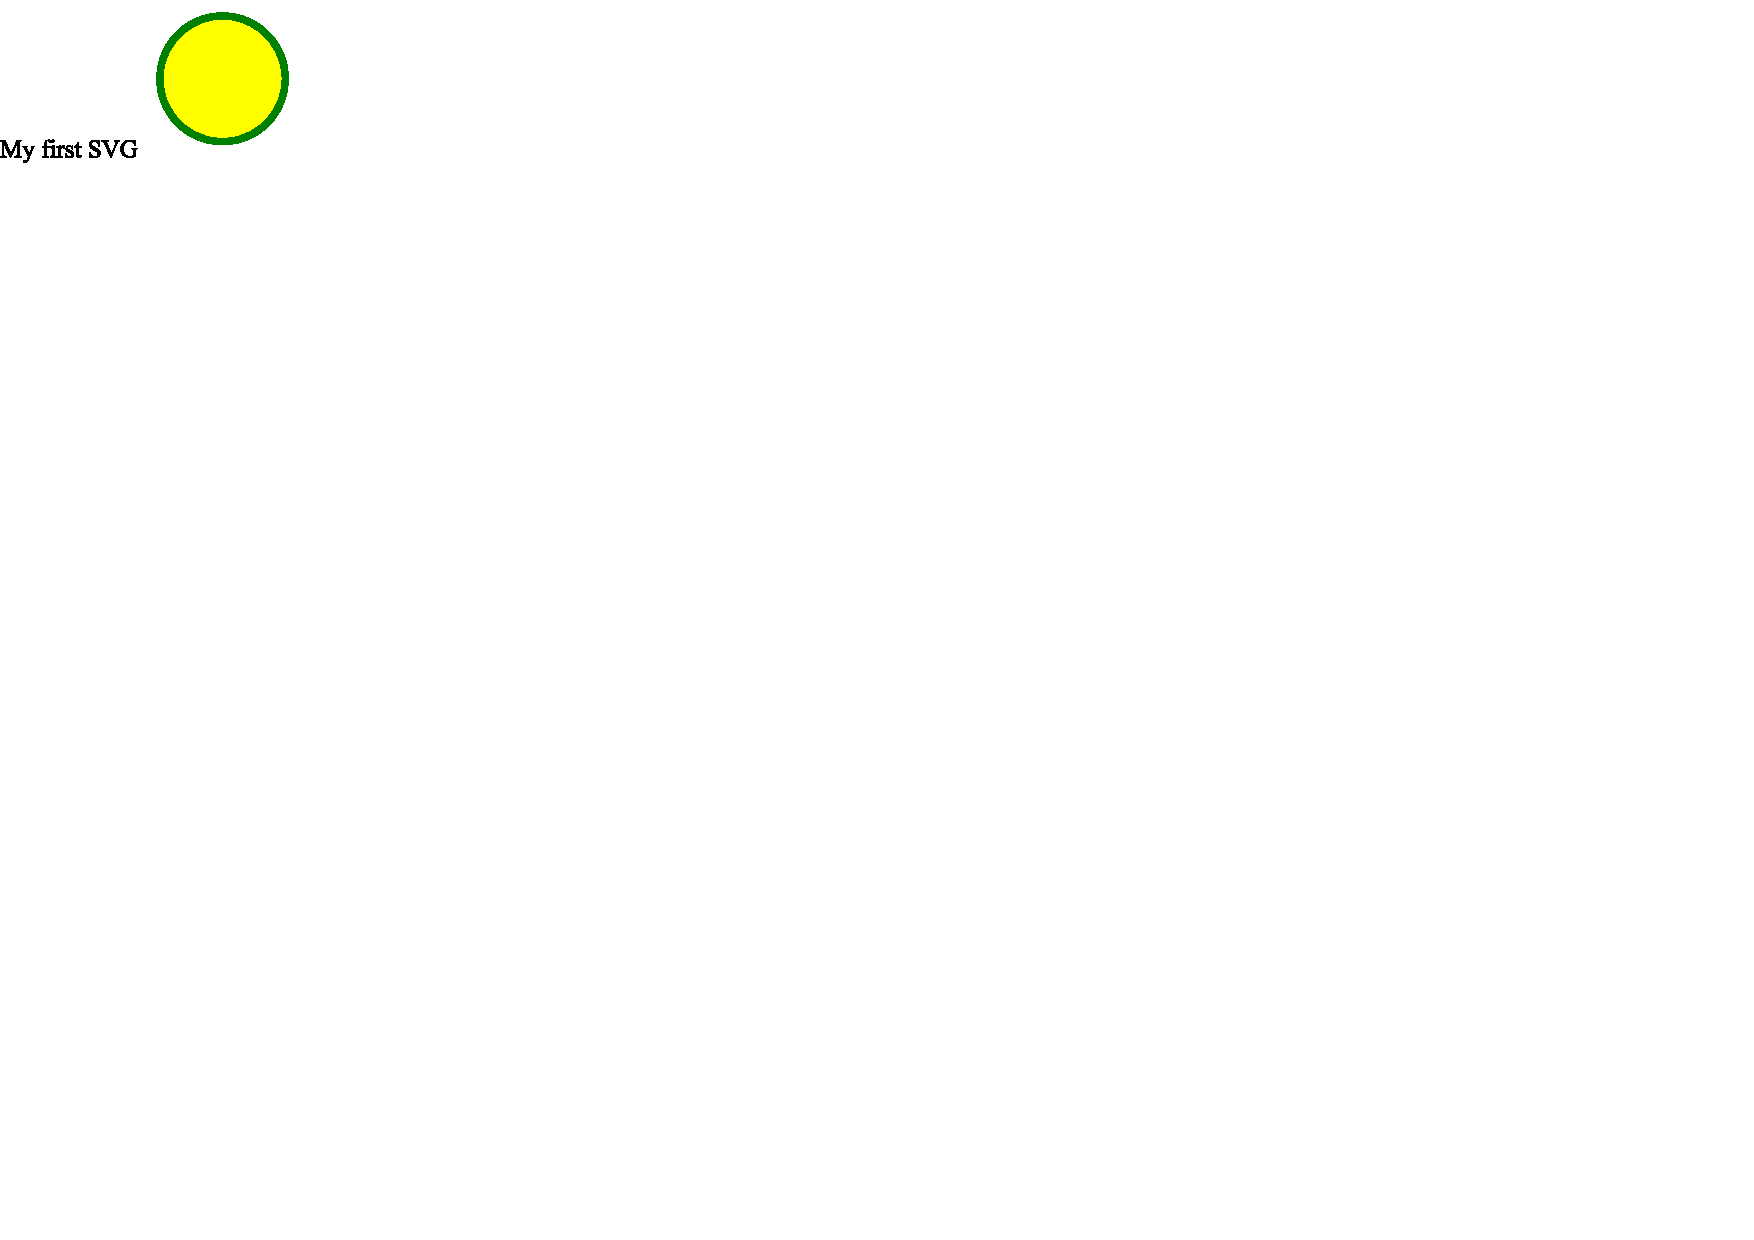
\includegraphics[width=\textwidth, angle=0]{Kreis2.pdf}
		\end{figure}
		\newpage
		\begin{figure}[h!]
		    \centering
		    \captionsetup{labelformat=empty}
		    \caption{Your caption}
		    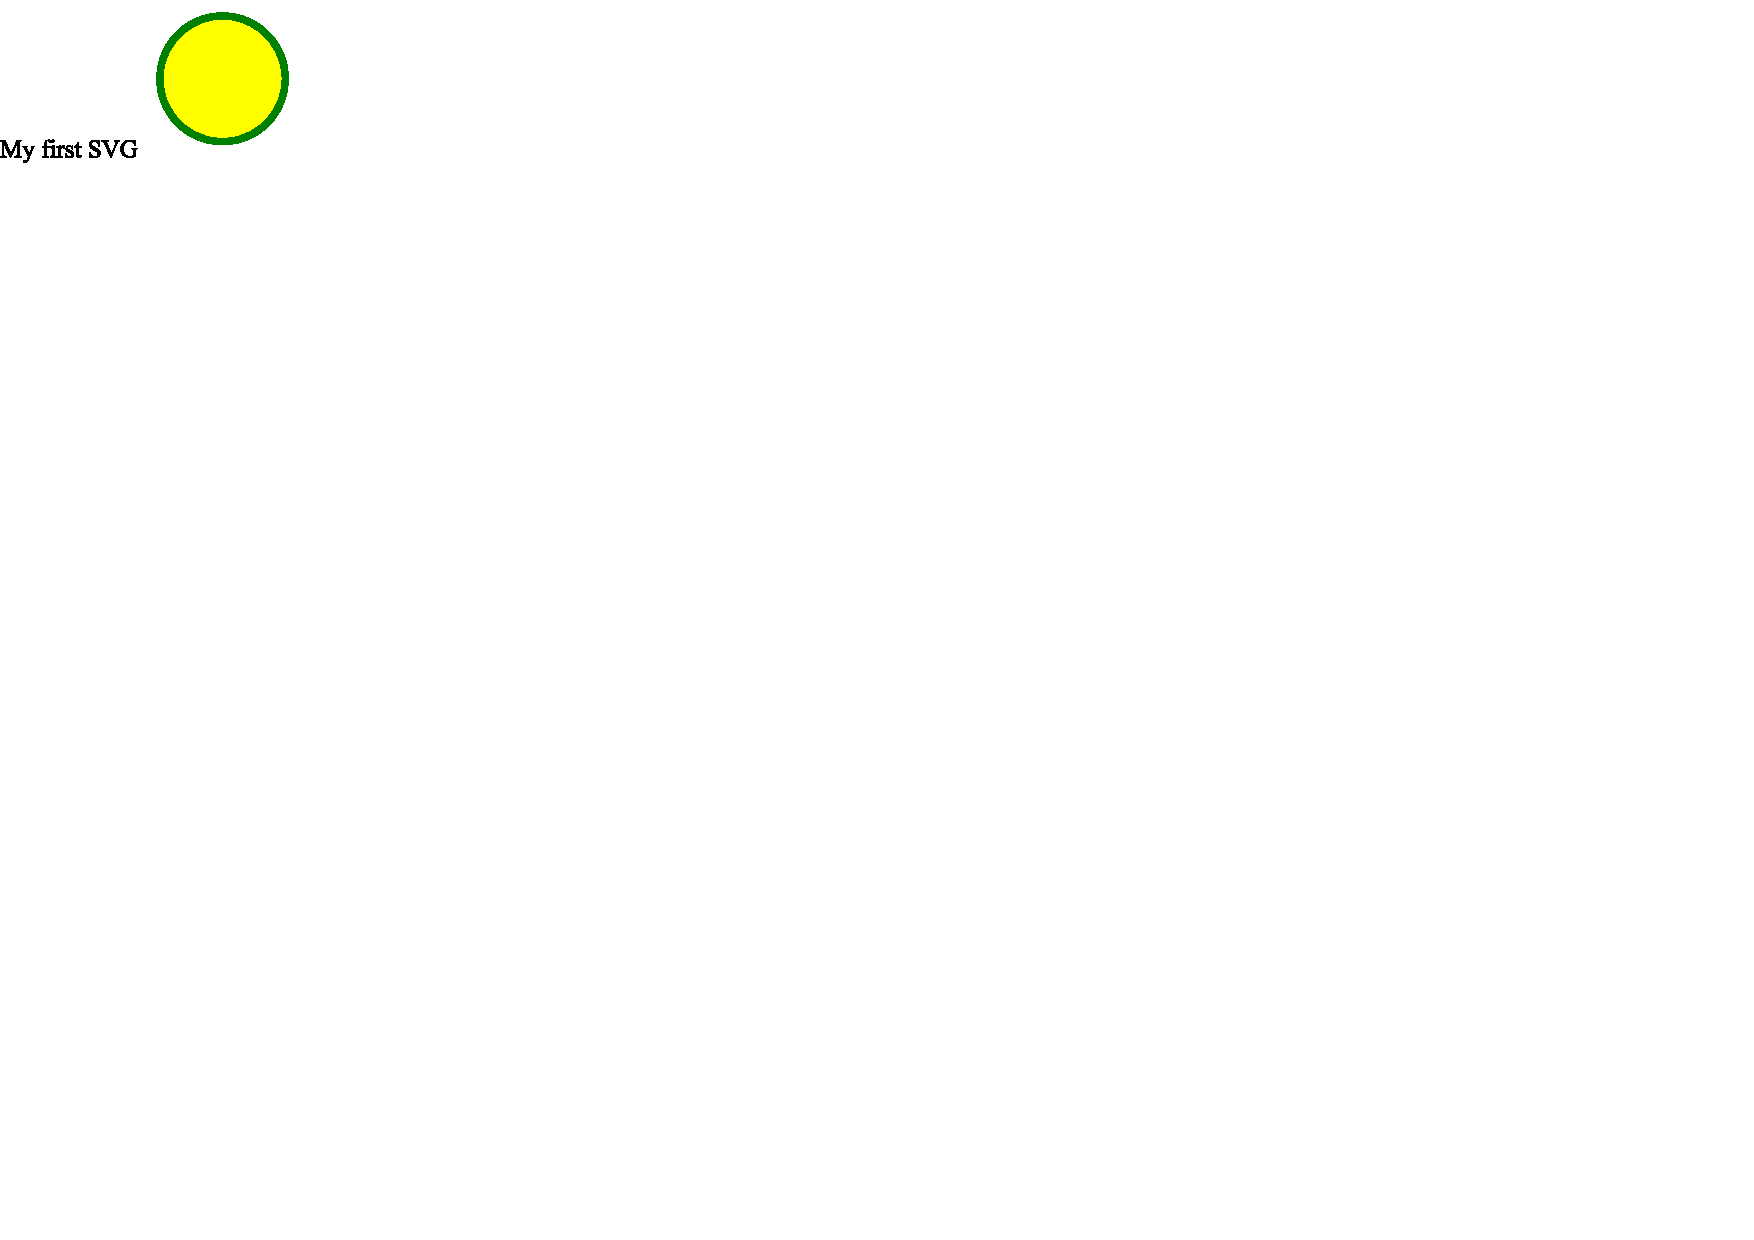
\includegraphics[width=\textwidth, angle=0]{Kreis2.pdf}
		\end{figure}
		\newpage



\section[]{Lars Friese}
	\subsection{Requirement 10: Easy usability with Gesture Control}
	\begin{center}
		\begin{tabularx}{1.0\textwidth}{|>{\raggedright\arraybackslash}p{0.2\textwidth}|>{\raggedright\arraybackslash}X|}
			\hline
			Name             & Use gestures to execute actions on smartwatch \\ \hline
			ID               & 12 \\ \hline
			Business Value   & medium \\ \hline
			Description      & When the user lifts his arm and turns his wrist the smartwatch display turns on, when he lowers the arm the display turns of. Additionally the smartwatch executes a costum gesture \\ \hline
			Trigger          & User lifting/lowering arm and turning wrist or shaking his wrist \\ \hline
			Actors           & User, System, Gyroscope Sensor\\ \hline
			Pre-conditions   & Display is turned on/off\\ \hline
			Post-conditions  & Display is turned on/off, App opened\\ \hline
			Basic Flow       & \\ \hline
							  Description & This is the main scenario where the system recognizes the hand up movement \\ \hline
							  Actions & \\ \hline
							  1 & User raises arm \\ \hline
							  2 & System recognizes gesture \\ \hline
							  3 & Display turns on \\ \hline
			Alternative Flow & A \\ \hline
							  Description & Actions \\ \hline
							  & 1 \\ \hline
							  & 2 \\ \hline
			Alternative Flow & B \\ \hline
							  Description & Actions \\ \hline
							  & 1 \\ \hline
							  & 2 \\ \hline
							  & 3 \\ \hline
							  & 4 \\ \hline
							  & 5 \\ \hline
		\end{tabularx}
	\end{center}

	\begin{figure}[htbp]
		\centering
		\begin{subfigure}{\textwidth}
			\resizebox{\textwidth}{!}{\includesvg[]{Lars/Use Case Gesture Control/GestureControl_usecase.svg}}
			\caption{Use Case Diagram}
		\end{subfigure}
		\begin{subfigure}{\textwidth}
			Example text 1 \
			Example text 2
		\end{subfigure}
	\end{figure}
	
	\begin{figure}[htbp]
		\centering
		\begin{subfigure}{\textwidth}
			\resizebox{\textwidth}{!}{\includesvg[]{Lars/Use Case Gesture Control/GestureControl_activity.svg}}
			\caption{Activity Diagram}
		\end{subfigure}
		\begin{subfigure}{\textwidth}
			Example text 3 \\
			Example text STARWBERRY 
		\end{subfigure}
	\end{figure}
	
	\begin{figure}[htbp]
		\centering
		\begin{subfigure}{\textwidth}
			\resizebox{\textwidth}{!}{\includesvg[]{Lars/Use Case Gesture Control/GestureControl_class.svg}}
			\caption{Class Diagram}
		\end{subfigure}
		\begin{subfigure}{\textwidth}
			Example text 5 \\
			Example text 6 
		\end{subfigure}
	\end{figure}
	
	\begin{figure}[htbp]
		\centering
		\begin{subfigure}{\textwidth}
			\resizebox{\textwidth}{!}{\includesvg[]{Lars/Use Case Gesture Control/GestureControl_sequence.svg}}
			\caption{Sequence Diagram}
		\end{subfigure}
		\begin{subfigure}{\textwidth}
			Example text 7 \\
			Example text 8
		\end{subfigure}
	\end{figure}
\newpage


\section{Marc Roemer}
	\subsection{Requirement 9: Calculation and display daily and weekly step count statistics}
		\begin{figure}[h!]
			\centering
			\captionsetup{labelformat=empty}
			\caption{UseCase}
		\end{figure}
		\newpage
		\begin{figure}[h!]
			\centering
			\captionsetup{labelformat=empty}
			\caption{UI Prototype}
		\end{figure}
		\newpage
		\begin{figure}[h!]
		    \centering
		    \captionsetup{labelformat=empty}
		    \caption{Activity Diagram}
		    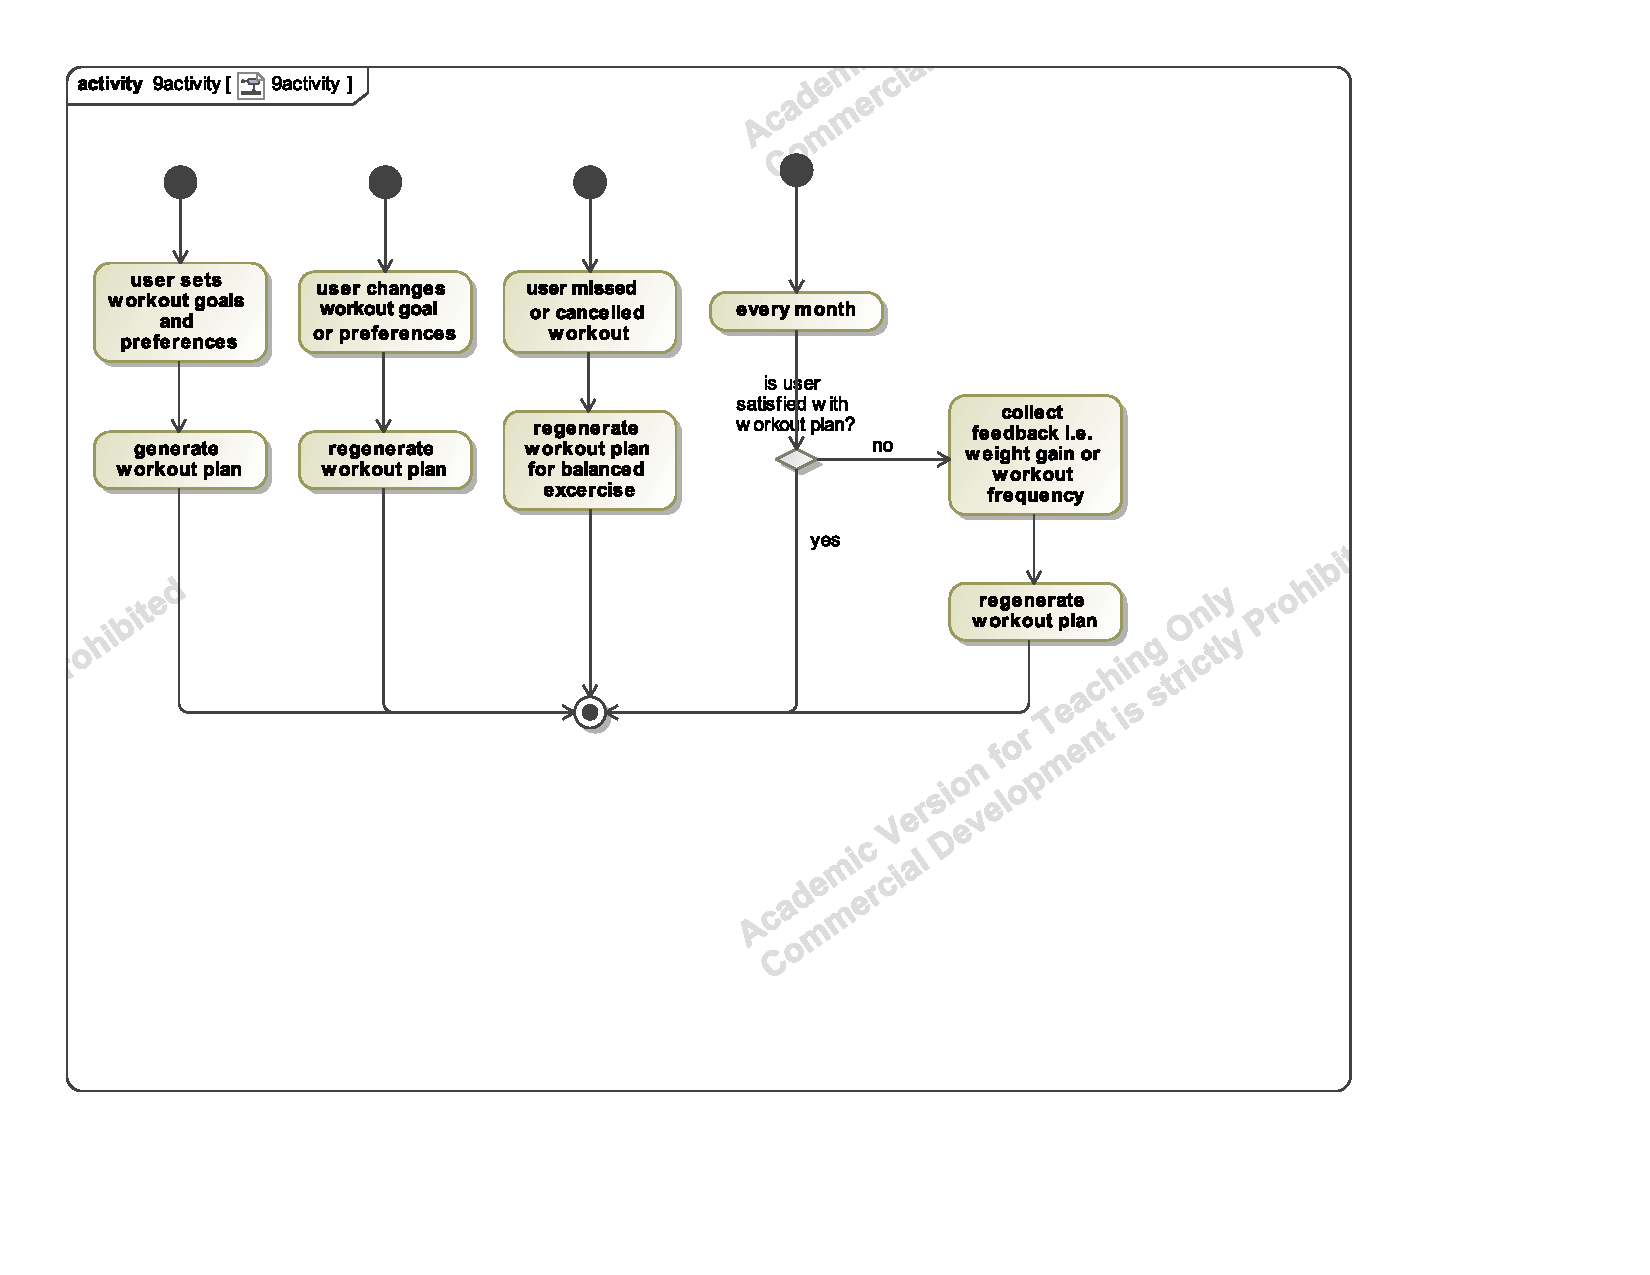
\includegraphics[width=\textwidth, angle=0]{Marc/req9/9activity.pdf}
		\end{figure}
		\newpage
		\begin{figure}[h!]
			\centering
			\captionsetup{labelformat=empty}
			\caption{UseCase Diagram}
		\end{figure}
		\newpage
		\begin{figure}[h!]
			\centering
			\captionsetup{labelformat=empty}
			\caption{Sequence Diagram}
		\end{figure}
		\newpage
		\begin{figure}[h!]
			\centering
			\captionsetup{labelformat=empty}
			\caption{Class Diagram}
		\end{figure}
		\newpage

	\subsection{Requirement 10: Create and manages a workout plan}
		\begin{figure}[h!]
			\centering
			\captionsetup{labelformat=empty}
			\caption{UseCase}
		\end{figure}
		\newpage
		\begin{figure}[h!]
			\centering
			\captionsetup{labelformat=empty}
			\caption{UI Prototype}
		\end{figure}
		\newpage
		\begin{figure}[h!]
		    \centering
		    \captionsetup{labelformat=empty}
		    \caption{Activity Diagram}
		    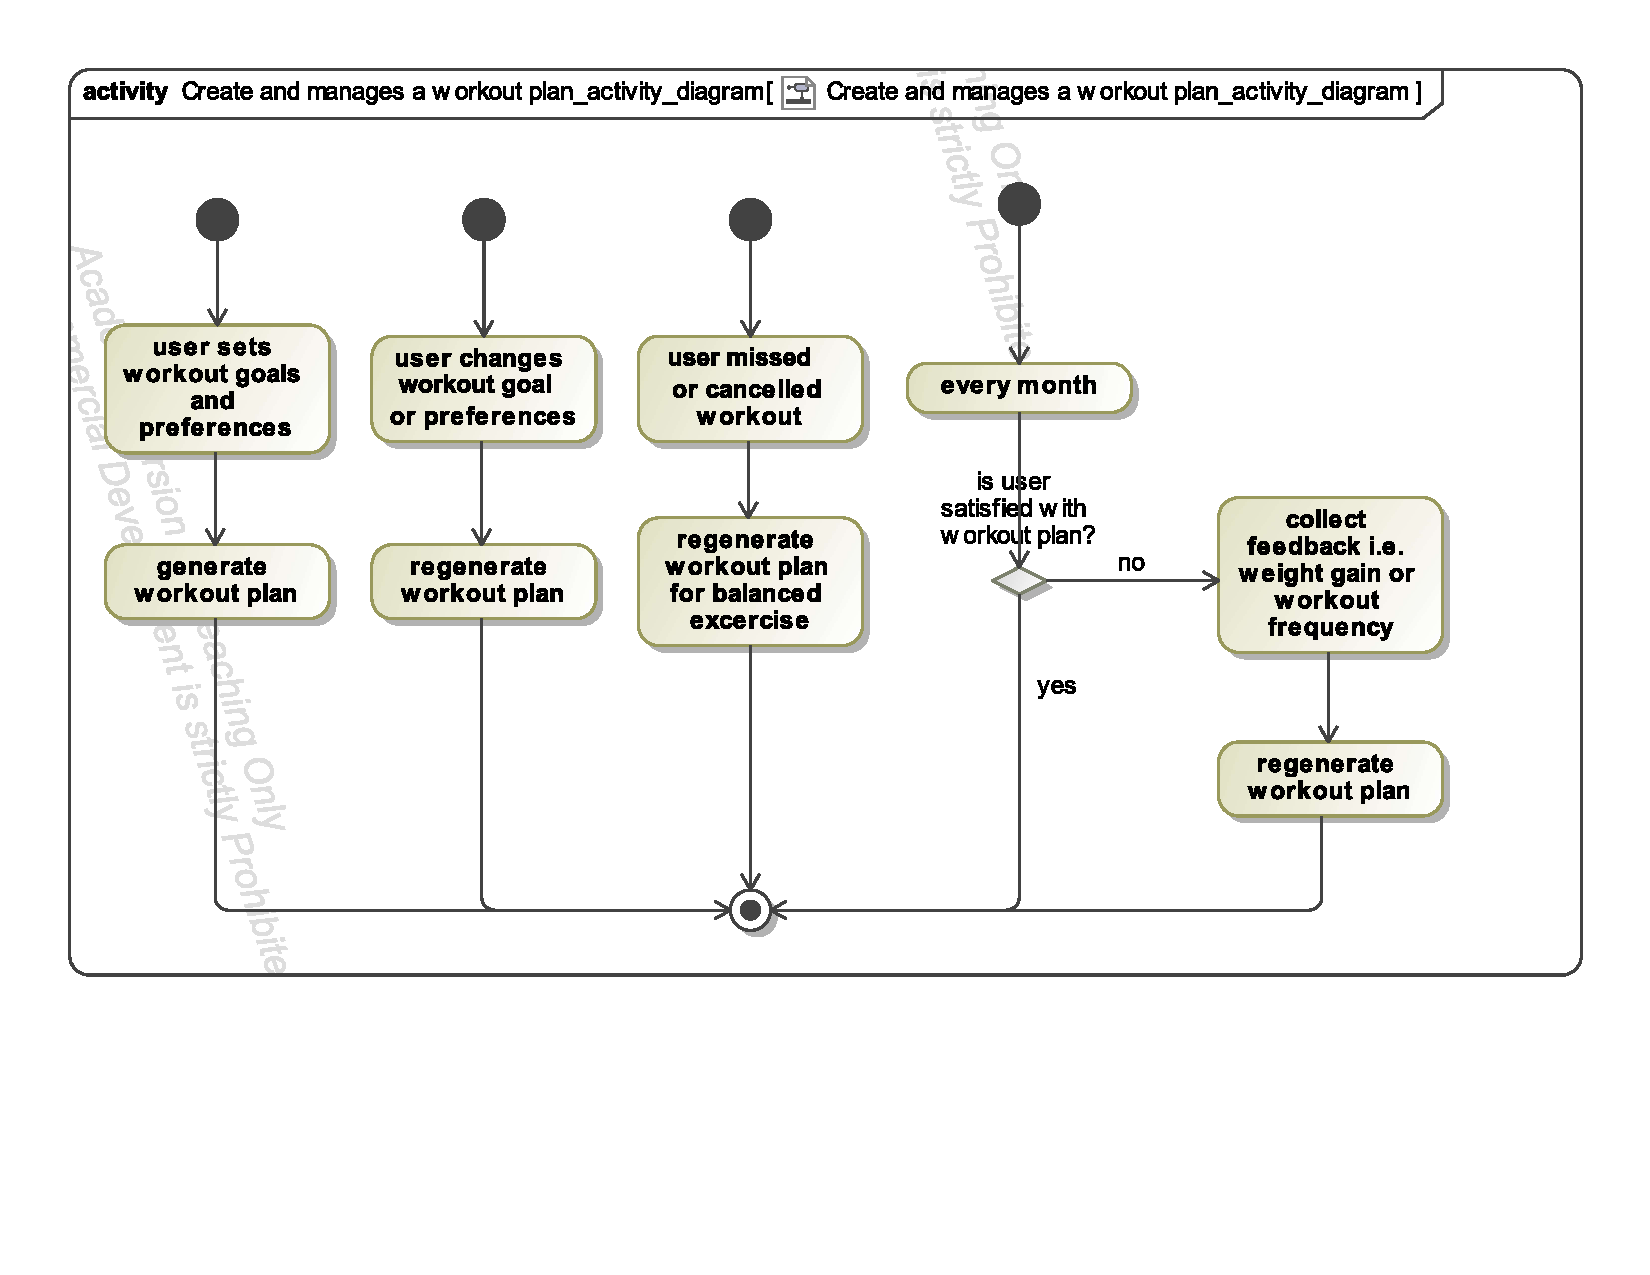
\includegraphics[width=\textwidth, angle=0]{Marc/req10/10activity.pdf}
		\end{figure}
		\newpage
		\begin{figure}[h!]
			\centering
			\captionsetup{labelformat=empty}
			\caption{UseCase Diagram}
		\end{figure}
		\newpage
		\begin{figure}[h!]
			\centering
			\captionsetup{labelformat=empty}
			\caption{Sequence Diagram}
		\end{figure}
		\newpage
		\begin{figure}[h!]
			\centering
			\captionsetup{labelformat=empty}
			\caption{Class Diagram}
		\end{figure}
		\newpage
			

\section{Stefan Nguyen}

\subsection{Requirement 3: Display Heart Rate on Smartwatch}
	\begin{center}
		\begin{tabularx}{1.0\textwidth}{|>{\raggedright\arraybackslash}p{0.2\textwidth}|>{\raggedright\arraybackslash}X|}
			\hline
			Name             & Display Heart Rate on Smartwatch \\ \hline
			ID               & 3 \\ \hline
			Business Value   & Medium \\ \hline
			Description      & User can look at their herat beat data on the smartwatch \\ \hline
			Trigger          & Click app icon from "health app" on smartwatch display, and then enter section "heart beat" \\ \hline
			Actors           & User, Health data app, Heartbeat sensor \\ \hline
			Pre-conditions   & Smartwatch turned on \\ \hline
			Post-conditions  & User receives information about his health data \\ \hline
			Basic Flow       & \\ \hline
							Description & This is the main scenario where the user already has a valid account and password \\ \hline
							Actions & \\ \hline
							1 & The user opens the heartbeat app \\ \hline
							2 & The app presents the user current heartrate in real time \\ \hline
			Alternative Flow & A \\ \hline
							Description & Inaccurate Sensoring of the heart beat \\ \hline
							Actions & \\ \hline
							1 & The app alerts the user about potential inaccuracy of the heart beat rate because of sensor issues. \\ \hline
							2 & The app guides the user through a recalibration of the sensor for accurate restults.  \\ \hline
			Alternative Flow & B \\ \hline
							Description & App sensors an anomaly in the heartbeat pattern  \\ \hline
							Actions & \\ \hline
							1 & The app sends a push notification to the user that the sensors detected an irregular heart beat. \\ \hline
							2 & The app provides guidance and relaxation techniques to normalize the heart beat rate. \\ \hline
							3 & If the heart beat doesn't change the app gives the user the possibility to call medical service. \\ \hline
		\end{tabularx}
	\end{center}


\begin{figure}[htbp]
	\centering
	\begin{subfigure}{\textwidth}
		\resizebox{\textwidth}{!}{\includesvg[]{Stefan/Display heart rate data on smartwatch/DisplayHeartRateDataOnSmartwatch_use_case_diagram.svg}}
		\caption{Use Case Diagram}
	\end{subfigure}
	\begin{subfigure}{\textwidth}
		The User has specific interactions for example he is able to review his heart rate on the history, he can also receive
		heart rate alerts which will include safety confirmation and extend if an emergency is needed. We can also set a limit of heart rate for example,
		if the user sets the limit to 140 bpm then he will get notified if we get passed that bpm. Next he can view the current heart rate on the smartwatch.
		The External health monioring service can sensor the heart rate proceed its data and give the user personal insight of his heartrate. 
	\end{subfigure}
\end{figure}


\begin{figure}[htbp]
	\centering
	\begin{subfigure}{\textwidth}
		\resizebox{\textwidth}{!}{\includesvg[]{Stefan/Display heart rate data on smartwatch/DisplayHeartRateDataOnSmartwatch_activity_diagram.svg}}
		\caption{Activity Diagram}
	\end{subfigure}
	\begin{subfigure}{\textwidth}
		Inside the Activity Diagram we start sensor the heart rate and proceed the data. Then with the given analysis it checks the 
		heart rate from the user. If its not fine we prepare an alert and send the user a safety confirmation. If its needed then we call an ambulance. If not 
		we can display the heartbeat data on the smartwatch. Then the user has a variety of options inside the smartwatch, e.g. 
		view current heart rate or the history of the past analysis or even receive personal insight of the heart rate. 
	\end{subfigure}
\end{figure}


\begin{figure}[htbp]
	\centering
	\begin{subfigure}{\textwidth}
		\resizebox{\textwidth}{!}{\includesvg[]{Stefan/Display heart rate data on smartwatch/DisplayHeartRateDataOnSmartwatch_class_diagram.svg}}
		\caption{Class Diagram}
	\end{subfigure}
	\begin{subfigure}{\textwidth}
		Inside the Class Diagram we check the data from the User because height, weight or even age does play an important factor
		for the heart rate analysis. Next we sensor the heart rate from the user and proceed the data. For that we use a directional 
		association since we do the operation once, and the muliplitiy stays 1 because we only use 1 sensor. Inside the process data we check for 
		the current heart rate. Last but not least, we display the data and the user is able to show the completed heart rate 
		analysis. 
	\end{subfigure}
\end{figure}


\begin{figure}[htbp]
	\centering
	\begin{subfigure}{\textwidth}
		\resizebox{\textwidth}{!}{\includesvg[]{Stefan/Display heart rate data on smartwatch/DisplayHeartRateDataOnSmartwatch_sequence_diagram.svg}}
		\caption{Sequence Diagram}
	\end{subfigure}
	\begin{subfigure}{\textwidth}
		Inside the Main we get the profile from the user and read the heartRate with the Sensor. Next we proceed the data and check 
		if a safety confirmation is needed. If yes we do an emergency call and we contact for medical assistance. Else we can process 
		the data and prepare to display the data to the user. When we send the data to the user we also make sure to stop the sensoring and 
		the user is able to review the current heart rate analysis. 
	\end{subfigure}
\end{figure}
\newpage

\subsection{Requirement 11: Environment Monitoring}
	\begin{center}
		\begin{tabularx}{1.0\textwidth}{|>{\raggedright\arraybackslash}p{0.2\textwidth}|>{\raggedright\arraybackslash}X|}
			\hline
			Name             & Environment monitoring \\ \hline
			ID               & 11 \\ \hline
			Business Value   & Low \\ \hline
			Description      & Tracks UV exposure, air quality, temperature in real time \\ \hline
			Trigger          & Typical event which adjusts the changes in real time \\ \hline
			Actors           & Environmental Sensor Array, which is responsible for capturing environmental data \\ \hline
			Pre-conditions   & Environmental sensors are operational and calibrated\\ \hline
			Post-conditions  & Displays the data in the smartwatch\\ \hline
			Basic Flow       & \\ \hline
							  Description & Detail each change in the environment monioring system \\ \hline
							  Actions & \\ \hline
							  1 & activating the sensors \\ \hline
							  2 & capturing the data (e.g. temperature, UV, etc) \\ \hline
							  3 & processing data e.g. analysis or computations \\ \hline
							  4 & transfer data into smartwatch \\ \hline
							  5 & display data in smartwatch \\ \hline
			Alternative Flow & A \\ \hline
							  Description & Error capturing data (network, communication etc) \\ \hline
							  Actions & \\ \hline
							  1 & sensor fails to capture data \\ \hline
							  2 & fail, communication or network error in smartwatch or sensor \\ \hline
							  3 & Error capturing data / false data display information \\ \hline
			Alternative Flow & B \\ \hline
							  Description & Environmental sensor detect conditions which my threaten health conditions \\ \hline
							  Actions & \\ \hline
							  1 & sensor detects hazardous condition and flag it as highest priority \\ \hline
							  2 & sends push notification and warns the user \\ \hline
							  3 & displays the notification on the smartwatch and recommends actions (e.g. apply sunscreen, seek shelter, etc) \\ \hline
							  4 & user acknowledges the notification\\ \hline
							  5 & user doesn't acknoweldege notification -> the system keeps sending notifications or warns the user \\ \hline
		\end{tabularx}
	\end{center}
	

	\begin{figure}[htbp]
		\centering
		\begin{subfigure}{\textwidth}
			\resizebox{\textwidth}{!}{\includesvg[]{Stefan/Environment Monitoring/EnvironmentMonitoring_use_case_diagram.svg}}
			\caption{Use Case Diagram}
		\end{subfigure}
		\begin{subfigure}{\textwidth}
			The Environment Monitoring shows the use cases. The Actvity sensor sensors the environment and transmit
			proceeds the data and generate a safe monioring notification. This tells the user the current environement e.g.
			temperature, UV exposure or more. If it comes to hazardous conditions it sends the user a notification and asks him 
			to either acknoweldege or not. Next the activity sensor displays the data on the smartwatch and record or
			track any other incident reports. The user on the other hand can acknoweldege the notification and look into
			history data and has an authentification. 
		\end{subfigure}
	\end{figure}
	

	\begin{figure}[htbp]
		\centering
		\begin{subfigure}{\textwidth}
			\resizebox{\textwidth}{!}{\includesvg[]{Stefan/Environment Monitoring/EnvironmentMonitoring_activity_diagram.svg}}
			\caption{Activity Diagram}
		\end{subfigure}
		\begin{subfigure}{\textwidth}
			The activity diagram shows a walkthrough of the operations or activities that need to be done, 
			so it can monitor the environment. Firstly, it activates the sensor and collects all the environment 
			data and transmits/proceeds them. It later asks for safe monitoring to ensure that there are no incidents 
			like hazards or natural disasters. If the user clicks no then the system prepares the notification and 
			asks the user to acknowledge the alert. The alert shows tips or recommendations which need to be done, to 
			shorten the risk of endangering personal life. If the user doesn’t accept the notification then the system 
			keeps warning the user or keeps spamming alerts, else it displays the data with the notification.
		\end{subfigure}
	\end{figure}
	

	\begin{figure}[htbp]
		\centering
		\begin{subfigure}{\textwidth}
			\resizebox{\textwidth}{!}{\includesvg[]{Stefan/Environment Monitoring/EnvironmentMonitoring_class_diagram.svg}}
			\caption{Class Diagram}
		\end{subfigure}
		\begin{subfigure}{\textwidth}
			The UML shows the structure of the classes, how they interact with each other and what methods are 
			used later in the sequence diagram. For example, the Activity Sensor sends data to the process data 
			which is a unidirectional relation with 1. The activity sensor has methods like activate sensor, keep 
			monitoring and stop monitoring. The monitoring would work permanently while the smartwatch is on. The 
			process list has the notifications, hazardous condition and process data and uses the unidirectional 
			relation to the display. While the display formats the data to the smartwatch so that the user can access 
			the data and can see the outputted data. 
		\end{subfigure}
	\end{figure}
	

	\begin{figure}[htbp]
		\centering
		\begin{subfigure}{\textwidth}
			\resizebox{\textwidth}{!}{\includesvg[]{Stefan/Environment Monitoring/EnvironmentMonitoring_sequence_diagram.svg}}
			\caption{Sequence Diagram}
		\end{subfigure}
		\begin{subfigure}{\textwidth}
			The sensor diagram almost works the same way as the display heartbeat data. It activates the sensor, 
			does the process and checks for hazardous conditions in the environment and does the following alternative
			operations. Later it either sends a notification or outputs the data to the display of the smartwatch. 
			The small part of smartwatch on represents that the sensor works permanently and keeps monitoring until 
			the smartwatch is off. 
		\end{subfigure}
	\end{figure}
	\newpage

\subsection{Requirement 13: Pay with Smartwatch}
	\begin{center}
		\begin{tabularx}{1.0\textwidth}{|>{\raggedright\arraybackslash}p{0.2\textwidth}|>{\raggedright\arraybackslash}X|}
			\hline
			Name             & Pay with Smartwatch \\ \hline
			ID               & 13 \\ \hline
			Business Value   & Low \\ \hline
			Description      & Allows users to make payments using their smartwatch connected to a digital wallet or bank account. \\ \hline
			Trigger          & User chooses to pay with a smartwatch within an app  \\ \hline
			Actors           & User, Payment System, Bank \\ \hline
			Pre-conditions   & smartwatch with payment capability, bank acount must be linked to digital wallet, the card reader supports the smartwatch payments \\ \hline
			Post-conditions  & process confirmed, receipt sent to user email, recorded to the transaction history \\ \hline
			Basic Flow       & \\ \hline
							Description & User completes the smartwatch transaction \\ \hline
							Actions & \\ \hline
							1 & Selects "Pay with Smartwatch" option within the app and reads with the card reader \\ \hline
							2 & User sees the amount to pay and confirms the payment  \\ \hline
							3 & Payment system processes the transaction with the user's bank or digitial wallet \\ \hline
							4 & confirmation through the card reader and receipt sent to the users email \\ \hline
			Alternative Flow & A \\ \hline
							Description & Payment with smartwatch fails due to connectivity issues \\ \hline
							Actions & \\ \hline
							1 & User attempts to pay, but the smartwatch cant connect to the card reader \\ \hline
							2 & The card reader sends an error message \\ \hline
							3 & User resolves the issue or decides to pay with a different payment method \\ \hline
			Alternative Flow & B \\ \hline
							Description & Payment declined by the bank or digital wallet \\ \hline
							Actions & \\ \hline
							1 & User confirms the payment on the smartwatch \\ \hline
							2 & Payment system processes the transaction but receives an error due wrong password  \\ \hline
							3 & User retry entering password but still no result \\ \hline
							4 & Bank account blocks the card \\ \hline
							5 & User gets notificated and needs to pay with a different payment method \\ \hline
		\end{tabularx}
	\end{center}


	\begin{figure}[htbp]
		\centering
		\begin{subfigure}{\textwidth}
			\resizebox{\textwidth}{!}{\includesvg[]{Stefan/Pay with Smartwatch/PayWithSmartwatch_use_case_diagram.svg}}
			\caption{Use Case Diagram}
		\end{subfigure}
		\begin{subfigure}{\textwidth}
			The Use Case Diagram describes the different connection and actions the user can do within the smartwatch. For example, 
			the user is able to pay with the smartwatch. After it reads the smartwatch in the card reader it verifies the card and 
			either complete the transaction or cancel the transaction. If the transaction completes the user gets a receipt or an 
			email which confirms the payment. In addition the user is able to manage his bank accounts inside the smartwatch application. 
		\end{subfigure}
	\end{figure}


	\begin{figure}[htbp]
		\centering
		\begin{subfigure}{\textwidth}
			\resizebox{\textwidth}{!}{\includesvg[]{Stefan/Pay with Smartwatch/PayWithSmartwatch_activity_diagram.svg}}
			\caption{Activity Diagram}
		\end{subfigure}
		\begin{subfigure}{\textwidth}
			The Activity Diagram describes the process of actions. For example the user holds his smartwatch with the digital card
			to a card reader and the card reader verifies if the card exists or does not. If the card doesn't exists it notifies
			the user that the card is invalid. Else we proceed to the bank account and the user should enter the password. If the 
			password is wrong it requests to enter the password again. After 3 tries it should automatically block the user. Else the 
			cash has been successfully transfered and the user can complete the transaction. 
		\end{subfigure}
	\end{figure}


	\begin{figure}[htbp]
		\centering
		\begin{subfigure}{\textwidth}
			\resizebox{\textwidth}{!}{\includesvg[]{Stefan/Pay with Smartwatch/PayWithSmartwatch_class_diagram.svg}}
			\caption{Class Diagram}
		\end{subfigure}
		\begin{subfigure}{\textwidth}
			The Class Diagram shows the interactions and relationships to each single process. For example, the User is
			able to create an account and register himself. Then it has a directional association to the proceed Data. Thats
			where the card is being checked, wheither it exists or not. If it exists we simply go to the bank account and check 
			for the password and get the receipt that the transaction was sucessful. If there is a case when the password is 
			incorrect we simply ask the user to retry. If the retries all failed or the user decides to pay with a different 
			payment method we need to stop the process. 
		\end{subfigure}
	\end{figure}
	\newpage

	\begin{figure}[htbp]
		\centering
		\begin{subfigure}{\textwidth}
			\resizebox{\textwidth}{!}{\includesvg[]{Stefan/Pay with Smartwatch/PayWithSmartwatch_sequence_diagram.svg}}
			\caption{Sequence Diagram}
		\end{subfigure}
		\begin{subfigure}{\textwidth}
			Inside the Sequence Diagram we have a Main which opens the smartwatch. Then the user checks the digital card with the 
			card reader if it exists or not. If it doesn't we simply stop the program. Else we can just check if its vaild and request the 
			user to enter the password. If the password is correct we get the receipt and the transaction message. If we might occur to incorrect 
			password we have 2 more retries and if those 2 failed aswell we stop the program if not we can get the receipt and the transaction
			message. 
		\end{subfigure}
	\end{figure}
	\newpage

\subsection{Requirement 14: Tips for using the Smartwatch}
	\begin{center}
		\begin{tabularx}{1.0\textwidth}{|>{\raggedright\arraybackslash}p{0.2\textwidth}|>{\raggedright\arraybackslash}X|}
			\hline
			Name             & Tips for using the Smartwatch \\ \hline
			ID               & 14 \\ \hline
			Business Value   & Low \\ \hline
			Description      & Provides the user with helpful tips and guidance throughout the smartwatch \\ \hline
			Trigger          & User requess tips and help with the smartwatch interface or associated app \\ \hline
			Actors           & User, Smartwatch, Companion smartwatch app \\ \hline
			Pre-conditions   & Smartwatch connected with phone, needs basic knowledge for the usage of the smartwatch \\ \hline
			Post-conditions  & User receives helpful tips and feels more confident using the smartwatch, engagement with the features increased \\ \hline
			Basic Flow       & \\ \hline
							Description & The user accesses and navigates through the tips inside the smartwatch application \\ \hline
							Actions & \\ \hline
							1 & User opens the tips feature and see the companion smartphone app \\ \hline
							2 & Browse through different categories like, fitness help or functionality throughout the watch \\ \hline
							3 & Selects the option \\ \hline
							4 & Enhance the smartwatch usage \\ \hline
			Alternative Flow & A \\ \hline
							Description & Connectivity error or fail opening the tips application \\ \hline
							Actions & \\ \hline
							1 & User attempts to access the tips application, but an error appeared due to connectivity errors. \\ \hline
							2 & Smartwatch prompts the user to check the internet connection  \\ \hline
							3 & User resolves the issue and can successfully enter the tips application \\ \hline
			Alternative Flow & B \\ \hline
							Description & User requests specific tips through a voice command, but the smartwatch does not recognize the command.  \\ \hline
							Actions & \\ \hline
							1 & User gives a voice command requesting tips on a specific feature \\ \hline
							2 & The smartwatch fails to recognize the command and asks the user to try again \\ \hline
							3 & User repeats the command with clearer pronunciation \\ \hline
							4 & If the smartwatch still fails to recognize the command, it asks to type the request \\ \hline
							5 & User types the request, and the smartwatch displays the relevant tips \\ \hline
		\end{tabularx}
	\end{center}
	

	\begin{figure}[htbp]
		\centering
		\begin{subfigure}{\textwidth}
			\resizebox{\textwidth}{!}{\includesvg[]{Stefan/Tips for using the Smartwatch/TipsUsingTheSmartwatch_use_case_diagram.svg}}
			\caption{Use Case Diagram}
		\end{subfigure}
		\begin{subfigure}{\textwidth}
			The Use Case Diagram for the Tips for using the smartwatch should just enhance the guidance for the user. So that the 
			user knows the new features of the smartwatch and help him get to know it better. So the user has the option to see a 
			variety of tips e.g. maintaining the device, customize the watch faces, smart notification and much more. Then if the user
			wants to find a specific tip there is also a search bar. Finally, the user can give feature advices inside the smartwatch
		\end{subfigure}
	\end{figure}
	
	\begin{figure}[htbp]
		\centering
		\begin{subfigure}{\textwidth}
			\resizebox{\textwidth}{!}{\includesvg[]{Stefan/Tips for using the Smartwatch/TipsUsingTheSmartwatch_activity_diagram.svg}}
			\caption{Activity Diagram}
		\end{subfigure}
		\begin{subfigure}{\textwidth}
			The Activity Diagram shows the process for using the tips application. It is required to open the smartwatch and 
			navigate to the application. Then the user has options. For example, he can open the preset of tips, else he can search
			for specific elements. If the element is not found we simply notify the user that it's not available. 
			If the user choose a tip for guidance we simply continue with reading the tip or else we can just close the process. 
		\end{subfigure}
	\end{figure}
	

	\begin{figure}[htbp]
		\centering
		\begin{subfigure}{\textwidth}
			\resizebox{\textwidth}{!}{\includesvg[]{Stefan/Tips for using the Smartwatch/TipsUsingTheSmartwatch_class_diagram.svg}}
			\caption{Class Diagram}
		\end{subfigure}
		\begin{subfigure}{\textwidth}
			For the Class Diagram we have 3 classes. The user, searchbar and then the tips application. The User usually 
			has an id for this smartwatch an account is registered with a name. If the user decides to pick one of the presets
			it directs him/her to the tipsApplication, where he can read the advice. Else if he decides to search for an element 
			we can find it and directs us to the tipsApplication. 
		\end{subfigure}
	\end{figure}


	\begin{figure}[htbp]
		\centering
		\begin{subfigure}{\textwidth}
			\resizebox{\textwidth}{!}{\includesvg[]{Stefan/Tips for using the Smartwatch/TipsUsingTheSmartwatch_sequence_diagram.svg}}
			\caption{Sequence Diagram}
		\end{subfigure}
		\begin{subfigure}{\textwidth}
			The Sequence Diagram shows the process of the application. For example the user has the application opened. Then it can
			either teake the presets which directs us to the tips application and gets us the output. Or else we can search the element. 
			If we search for the element, we check if its found or not. If not then we simply say that the element is not found and close the application. 
			The other option is that the user found the tip and gets the output. 
		\end{subfigure}
	\end{figure}
	\newpage


\end{document}